\documentclass[]{article}
\usepackage{lmodern}
\usepackage{amssymb,amsmath}
\usepackage{ifxetex,ifluatex}
\usepackage{fixltx2e} % provides \textsubscript
\ifnum 0\ifxetex 1\fi\ifluatex 1\fi=0 % if pdftex
  \usepackage[T1]{fontenc}
  \usepackage[utf8]{inputenc}
\else % if luatex or xelatex
  \ifxetex
    \usepackage{mathspec}
  \else
    \usepackage{fontspec}
  \fi
  \defaultfontfeatures{Ligatures=TeX,Scale=MatchLowercase}
\fi
% use upquote if available, for straight quotes in verbatim environments
\IfFileExists{upquote.sty}{\usepackage{upquote}}{}
% use microtype if available
\IfFileExists{microtype.sty}{%
\usepackage{microtype}
\UseMicrotypeSet[protrusion]{basicmath} % disable protrusion for tt fonts
}{}
\usepackage[margin=1in]{geometry}
\usepackage{hyperref}
\hypersetup{unicode=true,
            pdftitle={BIOL 416 R Tutorial 1 - Introduction to R},
            pdfauthor={Mairin Deith},
            pdfborder={0 0 0},
            breaklinks=true}
\urlstyle{same}  % don't use monospace font for urls
\usepackage{color}
\usepackage{fancyvrb}
\newcommand{\VerbBar}{|}
\newcommand{\VERB}{\Verb[commandchars=\\\{\}]}
\DefineVerbatimEnvironment{Highlighting}{Verbatim}{commandchars=\\\{\}}
% Add ',fontsize=\small' for more characters per line
\usepackage{framed}
\definecolor{shadecolor}{RGB}{248,248,248}
\newenvironment{Shaded}{\begin{snugshade}}{\end{snugshade}}
\newcommand{\KeywordTok}[1]{\textcolor[rgb]{0.13,0.29,0.53}{\textbf{#1}}}
\newcommand{\DataTypeTok}[1]{\textcolor[rgb]{0.13,0.29,0.53}{#1}}
\newcommand{\DecValTok}[1]{\textcolor[rgb]{0.00,0.00,0.81}{#1}}
\newcommand{\BaseNTok}[1]{\textcolor[rgb]{0.00,0.00,0.81}{#1}}
\newcommand{\FloatTok}[1]{\textcolor[rgb]{0.00,0.00,0.81}{#1}}
\newcommand{\ConstantTok}[1]{\textcolor[rgb]{0.00,0.00,0.00}{#1}}
\newcommand{\CharTok}[1]{\textcolor[rgb]{0.31,0.60,0.02}{#1}}
\newcommand{\SpecialCharTok}[1]{\textcolor[rgb]{0.00,0.00,0.00}{#1}}
\newcommand{\StringTok}[1]{\textcolor[rgb]{0.31,0.60,0.02}{#1}}
\newcommand{\VerbatimStringTok}[1]{\textcolor[rgb]{0.31,0.60,0.02}{#1}}
\newcommand{\SpecialStringTok}[1]{\textcolor[rgb]{0.31,0.60,0.02}{#1}}
\newcommand{\ImportTok}[1]{#1}
\newcommand{\CommentTok}[1]{\textcolor[rgb]{0.56,0.35,0.01}{\textit{#1}}}
\newcommand{\DocumentationTok}[1]{\textcolor[rgb]{0.56,0.35,0.01}{\textbf{\textit{#1}}}}
\newcommand{\AnnotationTok}[1]{\textcolor[rgb]{0.56,0.35,0.01}{\textbf{\textit{#1}}}}
\newcommand{\CommentVarTok}[1]{\textcolor[rgb]{0.56,0.35,0.01}{\textbf{\textit{#1}}}}
\newcommand{\OtherTok}[1]{\textcolor[rgb]{0.56,0.35,0.01}{#1}}
\newcommand{\FunctionTok}[1]{\textcolor[rgb]{0.00,0.00,0.00}{#1}}
\newcommand{\VariableTok}[1]{\textcolor[rgb]{0.00,0.00,0.00}{#1}}
\newcommand{\ControlFlowTok}[1]{\textcolor[rgb]{0.13,0.29,0.53}{\textbf{#1}}}
\newcommand{\OperatorTok}[1]{\textcolor[rgb]{0.81,0.36,0.00}{\textbf{#1}}}
\newcommand{\BuiltInTok}[1]{#1}
\newcommand{\ExtensionTok}[1]{#1}
\newcommand{\PreprocessorTok}[1]{\textcolor[rgb]{0.56,0.35,0.01}{\textit{#1}}}
\newcommand{\AttributeTok}[1]{\textcolor[rgb]{0.77,0.63,0.00}{#1}}
\newcommand{\RegionMarkerTok}[1]{#1}
\newcommand{\InformationTok}[1]{\textcolor[rgb]{0.56,0.35,0.01}{\textbf{\textit{#1}}}}
\newcommand{\WarningTok}[1]{\textcolor[rgb]{0.56,0.35,0.01}{\textbf{\textit{#1}}}}
\newcommand{\AlertTok}[1]{\textcolor[rgb]{0.94,0.16,0.16}{#1}}
\newcommand{\ErrorTok}[1]{\textcolor[rgb]{0.64,0.00,0.00}{\textbf{#1}}}
\newcommand{\NormalTok}[1]{#1}
\usepackage{graphicx,grffile}
\makeatletter
\def\maxwidth{\ifdim\Gin@nat@width>\linewidth\linewidth\else\Gin@nat@width\fi}
\def\maxheight{\ifdim\Gin@nat@height>\textheight\textheight\else\Gin@nat@height\fi}
\makeatother
% Scale images if necessary, so that they will not overflow the page
% margins by default, and it is still possible to overwrite the defaults
% using explicit options in \includegraphics[width, height, ...]{}
\setkeys{Gin}{width=\maxwidth,height=\maxheight,keepaspectratio}
\IfFileExists{parskip.sty}{%
\usepackage{parskip}
}{% else
\setlength{\parindent}{0pt}
\setlength{\parskip}{6pt plus 2pt minus 1pt}
}
\setlength{\emergencystretch}{3em}  % prevent overfull lines
\providecommand{\tightlist}{%
  \setlength{\itemsep}{0pt}\setlength{\parskip}{0pt}}
\setcounter{secnumdepth}{0}
% Redefines (sub)paragraphs to behave more like sections
\ifx\paragraph\undefined\else
\let\oldparagraph\paragraph
\renewcommand{\paragraph}[1]{\oldparagraph{#1}\mbox{}}
\fi
\ifx\subparagraph\undefined\else
\let\oldsubparagraph\subparagraph
\renewcommand{\subparagraph}[1]{\oldsubparagraph{#1}\mbox{}}
\fi

%%% Use protect on footnotes to avoid problems with footnotes in titles
\let\rmarkdownfootnote\footnote%
\def\footnote{\protect\rmarkdownfootnote}

%%% Change title format to be more compact
\usepackage{titling}

% Create subtitle command for use in maketitle
\newcommand{\subtitle}[1]{
  \posttitle{
    \begin{center}\large#1\end{center}
    }
}

\setlength{\droptitle}{-2em}

  \title{BIOL 416 R Tutorial 1 - Introduction to R}
    \pretitle{\vspace{\droptitle}\centering\huge}
  \posttitle{\par}
    \author{Mairin Deith}
    \preauthor{\centering\large\emph}
  \postauthor{\par}
    \date{}
    \predate{}\postdate{}
  

\begin{document}
\maketitle

\section{Preface}\label{preface}

These tutorials were developed to teach high-level undergraduate
students the fundamentals of working in R and R Studio. Instructions
have been modified from Dr.~Steven Kembel's
\href{http://kembellab.ca/r-workshop/biodivR/SK_Biodiversity_R.html}{``Biodiversity
analysis in R'' walkthrough} to reflect the learning objectives of BIOL
416 at the University of British Columbia.

\section{Tutorial 1}\label{tutorial-1}

January 14 \& 16, 2019

\subsection{Prep}\label{prep}

Students should download the example iris.csv file from Canvas - this
will be used to read in with \texttt{read.csv()}.

\subsection{Working in RStudio and R}\label{working-in-rstudio-and-r}

Quick notes:

\begin{itemize}
\tightlist
\item
  the console communicates with the computer directly
\item
  For example: \texttt{\textgreater{}\ 1+1} does the math for you
\item
  workflow between the script pane and the console is possible with
  Ctrl-Enter (Windows/Linux) or Cmd-Enter (MacOS)
\item
  comments, lines starting with \texttt{\#} are ignored by the computer
  and can keep track of notes for yourself or other people that might
  look at your code
\item
  For example, what lines of code do, why you use certain functions,
  etc.
\end{itemize}

\subsection{Objects}\label{objects}

\textbf{Note: this does not currently include any introduction to lists,
this may be necessary depending on how much understanding of lists is
required to use the \texttt{picante} package and phylogenies in R.}

\subsubsection{0-dimensional objects (single
variables)}\label{dimensional-objects-single-variables}

The simplest objects in R are single values, or variables.

You assign a value to an object using \texttt{\textless{}-} notation.
For example, to create a variable called \texttt{x} that is equal to 5:

\begin{Shaded}
\begin{Highlighting}[]
\NormalTok{x <-}\StringTok{ }\DecValTok{5}
\end{Highlighting}
\end{Shaded}

A 0-dimensional object contains a single datum - a number, string of
text, logical TRUE or FALSE values, or other types. We'll explore each
of these later.

You can name these objects whatever you want, but be careful:
capitalization matters and you can't put spaces in the names.

It's generally a good idea to give the objects names that mean something
to you:

\begin{Shaded}
\begin{Highlighting}[]
\NormalTok{species.name <-}\StringTok{ "Homo sapiens"}
\NormalTok{am.i.human <-}\StringTok{ }\OtherTok{TRUE}
\NormalTok{number.of.legs <-}\StringTok{ }\DecValTok{2}
\end{Highlighting}
\end{Shaded}

Once you create an object, you can see what value it holds by calling
it:

\begin{Shaded}
\begin{Highlighting}[]
\NormalTok{x}
\end{Highlighting}
\end{Shaded}

\begin{verbatim}
## [1] 5
\end{verbatim}

\begin{Shaded}
\begin{Highlighting}[]
\NormalTok{species.name}
\end{Highlighting}
\end{Shaded}

\begin{verbatim}
## [1] "Homo sapiens"
\end{verbatim}

You can also re-write a variable by re-assigning a value to it:

\begin{Shaded}
\begin{Highlighting}[]
\NormalTok{x <-}\StringTok{ "new x"}
\NormalTok{x}
\end{Highlighting}
\end{Shaded}

\begin{verbatim}
## [1] "new x"
\end{verbatim}

\subsubsection{1-dimensional objects
(vectors)}\label{dimensional-objects-vectors}

It is also possible to make objects that have more than one value in
them.

Vectors are objects that contain multiple single datum, all in a row.
It's the same as vectors in matrix mathematics - a one-dimensional row
of values.

To make this vector:
\(v = \begin{pmatrix} 0 & 3 & 5 & 10 & 2 \end{pmatrix}\), we would
write:

\begin{Shaded}
\begin{Highlighting}[]
\NormalTok{v <-}\StringTok{ }\KeywordTok{c}\NormalTok{(}\DecValTok{0}\NormalTok{, }\DecValTok{3}\NormalTok{, }\DecValTok{5}\NormalTok{, }\DecValTok{10}\NormalTok{, }\DecValTok{2}\NormalTok{)}
\NormalTok{v}
\end{Highlighting}
\end{Shaded}

\begin{verbatim}
## [1]  0  3  5 10  2
\end{verbatim}

The \texttt{c()} here stands for combine.

There are a few ways to pull out a single value from your vector. First,
you can use square brackets (\texttt{{[}X{]}}, where \texttt{X} is a
number indicating the position where the datum you want is stored, from
1 to however many objects are in your vector).

\begin{Shaded}
\begin{Highlighting}[]
\NormalTok{v[}\DecValTok{1}\NormalTok{]}
\end{Highlighting}
\end{Shaded}

\begin{verbatim}
## [1] 0
\end{verbatim}

\begin{Shaded}
\begin{Highlighting}[]
\NormalTok{v[}\DecValTok{4}\NormalTok{]}
\end{Highlighting}
\end{Shaded}

\begin{verbatim}
## [1] 10
\end{verbatim}

\begin{Shaded}
\begin{Highlighting}[]
\NormalTok{v[}\DecValTok{10}\NormalTok{]}
\end{Highlighting}
\end{Shaded}

\begin{verbatim}
## [1] NA
\end{verbatim}

Because we don't have 10 datum in the vector, trying to pull out the
10th item gives \texttt{NA}, not applicable. The spot is empty.

We can also pull out multiple datum using \texttt{c()}, as before, or by
using \texttt{:}. The colon indicates to R that we want values across a
range; e.g. \texttt{1:3} means all numbers between 1 and 3
(\texttt{1,2,3}).

\begin{Shaded}
\begin{Highlighting}[]
\CommentTok{# Using the combine function:}
\NormalTok{v[}\KeywordTok{c}\NormalTok{(}\DecValTok{1}\NormalTok{,}\DecValTok{2}\NormalTok{)]}
\end{Highlighting}
\end{Shaded}

\begin{verbatim}
## [1] 0 3
\end{verbatim}

\begin{Shaded}
\begin{Highlighting}[]
\CommentTok{# Using a range of numbers:}
\NormalTok{v[}\DecValTok{1}\OperatorTok{:}\DecValTok{3}\NormalTok{]}
\end{Highlighting}
\end{Shaded}

\begin{verbatim}
## [1] 0 3 5
\end{verbatim}

Another way to pull out datum from a vector is by naming each object in
the vector, and referring to each datum by name rather than location:

\begin{Shaded}
\begin{Highlighting}[]
\KeywordTok{names}\NormalTok{(v) <-}\StringTok{ }\KeywordTok{c}\NormalTok{(}\StringTok{"One"}\NormalTok{,}\StringTok{"Two"}\NormalTok{,}\StringTok{"Three"}\NormalTok{,}\StringTok{"Four"}\NormalTok{,}\StringTok{"Five"}\NormalTok{)}
\CommentTok{# Now v has names attached to it}
\NormalTok{v[}\StringTok{"One"}\NormalTok{]}
\end{Highlighting}
\end{Shaded}

\begin{verbatim}
## One 
##   0
\end{verbatim}

\subsubsection{An aside on data classes}\label{an-aside-on-data-classes}

R uses three main types of classes:

\begin{itemize}
\tightlist
\item
  Numeric (numbers)
\item
  Strings (text or individual characters, denoted by including
  \texttt{"\ "} around the text)
\item
  Logical (also called Boolean, this class of data is a binary TRUE or
  FALSE value)
\end{itemize}

In a vector, all of the data have to be of the same type (numbers, text
strings, TRUE/FALSE) or else R will convert each datum to be some
universal type.

\begin{Shaded}
\begin{Highlighting}[]
\NormalTok{bad.v <-}\StringTok{ }\KeywordTok{c}\NormalTok{(}\DecValTok{0}\NormalTok{, }\StringTok{"twelve"}\NormalTok{, }\OtherTok{TRUE}\NormalTok{)}
\NormalTok{bad.v}
\end{Highlighting}
\end{Shaded}

\begin{verbatim}
## [1] "0"      "twelve" "TRUE"
\end{verbatim}

Notice that now R sees all of these as text strings - you can tell by
the \texttt{""}.

Let's try another example:

\begin{Shaded}
\begin{Highlighting}[]
\NormalTok{another.bad.v <-}\StringTok{ }\KeywordTok{c}\NormalTok{(}\DecValTok{0}\NormalTok{, }\OtherTok{TRUE}\NormalTok{, }\OtherTok{FALSE}\NormalTok{)}
\NormalTok{another.bad.v}
\end{Highlighting}
\end{Shaded}

\begin{verbatim}
## [1] 0 1 0
\end{verbatim}

In this case, R transformed the \texttt{TRUE} and \texttt{FALSE} values
into 0 and 1. This is because it is forcing the data to be of the same
class.

\subsubsection{2-dimensional objects (matrices and
dataframes)}\label{dimensional-objects-matrices-and-dataframes}

Most of the data that we're used to looking at comes in the form of a
table - the sort of data you would enter into a spreadsheet such that
you have observations in rows and attributes of those observations in
columns. Here's an example of a 2D data-set that comes automatically
with R - this is from the pre-loaded data-set called \texttt{iris}:

\begin{Shaded}
\begin{Highlighting}[]
\CommentTok{# Ignore this for now:}

\CommentTok{# Load in the pre-loaded iris dataset}
\KeywordTok{data}\NormalTok{(}\StringTok{'iris'}\NormalTok{)}
\KeywordTok{head}\NormalTok{(iris)}
\end{Highlighting}
\end{Shaded}

\begin{verbatim}
##   Sepal.Length Sepal.Width Petal.Length Petal.Width Species
## 1          5.1         3.5          1.4         0.2  setosa
## 2          4.9         3.0          1.4         0.2  setosa
## 3          4.7         3.2          1.3         0.2  setosa
## 4          4.6         3.1          1.5         0.2  setosa
## 5          5.0         3.6          1.4         0.2  setosa
## 6          5.4         3.9          1.7         0.4  setosa
\end{verbatim}

\begin{Shaded}
\begin{Highlighting}[]
\CommentTok{# Also demonstrate:}
\CommentTok{# View(iris)}
\end{Highlighting}
\end{Shaded}

Notice that when we use \texttt{data()} to load in the \texttt{iris}
data-set, the Environment has a new entry, \texttt{iris}. We'll talk
about what the \texttt{data()} command is in a minute - for now, just
look at how the data are put together:

\begin{itemize}
\tightlist
\item
  each column is a variable - ALL THE SAME TYPE!
\item
  each row is an observation
\end{itemize}

\texttt{data.frame}s can hold any type of data: numbers, text, or
factors. Each column contains the same type of data.

\begin{Shaded}
\begin{Highlighting}[]
\KeywordTok{class}\NormalTok{(iris)}
\end{Highlighting}
\end{Shaded}

\begin{verbatim}
## [1] "data.frame"
\end{verbatim}

Just like in 1-dimensional vectors, we can pull individual objects out
of the iris data-set using matrix notation.

\begin{Shaded}
\begin{Highlighting}[]
\CommentTok{# To pull out the object in row 1, column 1:}
\NormalTok{### Row first, then column}
\NormalTok{iris[}\DecValTok{1}\NormalTok{,}\DecValTok{1}\NormalTok{] }\CommentTok{# Note the "," separating the row}
\end{Highlighting}
\end{Shaded}

\begin{verbatim}
## [1] 5.1
\end{verbatim}

\begin{Shaded}
\begin{Highlighting}[]
\CommentTok{# To pull out a single column, leave the row spot empty...}
\NormalTok{iris[,}\DecValTok{1}\NormalTok{]}
\end{Highlighting}
\end{Shaded}

\begin{verbatim}
##   [1] 5.1 4.9 4.7 4.6 5.0 5.4 4.6 5.0 4.4 4.9 5.4 4.8 4.8 4.3 5.8 5.7 5.4
##  [18] 5.1 5.7 5.1 5.4 5.1 4.6 5.1 4.8 5.0 5.0 5.2 5.2 4.7 4.8 5.4 5.2 5.5
##  [35] 4.9 5.0 5.5 4.9 4.4 5.1 5.0 4.5 4.4 5.0 5.1 4.8 5.1 4.6 5.3 5.0 7.0
##  [52] 6.4 6.9 5.5 6.5 5.7 6.3 4.9 6.6 5.2 5.0 5.9 6.0 6.1 5.6 6.7 5.6 5.8
##  [69] 6.2 5.6 5.9 6.1 6.3 6.1 6.4 6.6 6.8 6.7 6.0 5.7 5.5 5.5 5.8 6.0 5.4
##  [86] 6.0 6.7 6.3 5.6 5.5 5.5 6.1 5.8 5.0 5.6 5.7 5.7 6.2 5.1 5.7 6.3 5.8
## [103] 7.1 6.3 6.5 7.6 4.9 7.3 6.7 7.2 6.5 6.4 6.8 5.7 5.8 6.4 6.5 7.7 7.7
## [120] 6.0 6.9 5.6 7.7 6.3 6.7 7.2 6.2 6.1 6.4 7.2 7.4 7.9 6.4 6.3 6.1 7.7
## [137] 6.3 6.4 6.0 6.9 6.7 6.9 5.8 6.8 6.7 6.7 6.3 6.5 6.2 5.9
\end{verbatim}

\begin{Shaded}
\begin{Highlighting}[]
\CommentTok{#...or use its name with a "$"}
\NormalTok{iris}\OperatorTok{$}\NormalTok{Sepal.Length}
\end{Highlighting}
\end{Shaded}

\begin{verbatim}
##   [1] 5.1 4.9 4.7 4.6 5.0 5.4 4.6 5.0 4.4 4.9 5.4 4.8 4.8 4.3 5.8 5.7 5.4
##  [18] 5.1 5.7 5.1 5.4 5.1 4.6 5.1 4.8 5.0 5.0 5.2 5.2 4.7 4.8 5.4 5.2 5.5
##  [35] 4.9 5.0 5.5 4.9 4.4 5.1 5.0 4.5 4.4 5.0 5.1 4.8 5.1 4.6 5.3 5.0 7.0
##  [52] 6.4 6.9 5.5 6.5 5.7 6.3 4.9 6.6 5.2 5.0 5.9 6.0 6.1 5.6 6.7 5.6 5.8
##  [69] 6.2 5.6 5.9 6.1 6.3 6.1 6.4 6.6 6.8 6.7 6.0 5.7 5.5 5.5 5.8 6.0 5.4
##  [86] 6.0 6.7 6.3 5.6 5.5 5.5 6.1 5.8 5.0 5.6 5.7 5.7 6.2 5.1 5.7 6.3 5.8
## [103] 7.1 6.3 6.5 7.6 4.9 7.3 6.7 7.2 6.5 6.4 6.8 5.7 5.8 6.4 6.5 7.7 7.7
## [120] 6.0 6.9 5.6 7.7 6.3 6.7 7.2 6.2 6.1 6.4 7.2 7.4 7.9 6.4 6.3 6.1 7.7
## [137] 6.3 6.4 6.0 6.9 6.7 6.9 5.8 6.8 6.7 6.7 6.3 6.5 6.2 5.9
\end{verbatim}

\begin{Shaded}
\begin{Highlighting}[]
\CommentTok{# To pull out a single row, leave the column spot empty:}
\NormalTok{iris[}\DecValTok{1}\NormalTok{,]}
\end{Highlighting}
\end{Shaded}

\begin{verbatim}
##   Sepal.Length Sepal.Width Petal.Length Petal.Width Species
## 1          5.1         3.5          1.4         0.2  setosa
\end{verbatim}

\begin{Shaded}
\begin{Highlighting}[]
\CommentTok{# Don't forget that if you want to use a subset of the total data.frame later, you can save any of these as its own variable}
\NormalTok{sep.length <-}\StringTok{ }\NormalTok{iris}\OperatorTok{$}\NormalTok{Sepal.Length}

\CommentTok{# Ask: any guesses about what type of object this will be?}
\KeywordTok{class}\NormalTok{(sep.length)}
\end{Highlighting}
\end{Shaded}

\begin{verbatim}
## [1] "numeric"
\end{verbatim}

\subsection{Modifying variables}\label{modifying-variables}

To modify numeric variables, you can re-save the variable with the same
name\ldots{}

\begin{Shaded}
\begin{Highlighting}[]
\NormalTok{x <-}\StringTok{ }\DecValTok{5}
\NormalTok{x <-}\StringTok{ }\NormalTok{x}\OperatorTok{+}\DecValTok{3}
\NormalTok{x}
\end{Highlighting}
\end{Shaded}

\begin{verbatim}
## [1] 8
\end{verbatim}

\ldots{}you can make the object larger by turning a single number into a
list of numbers\ldots{}

\begin{Shaded}
\begin{Highlighting}[]
\NormalTok{x <-}\StringTok{ }\KeywordTok{c}\NormalTok{(x,}\DecValTok{5}\NormalTok{,}\DecValTok{12}\NormalTok{,}\DecValTok{15}\NormalTok{)}
\NormalTok{x}
\end{Highlighting}
\end{Shaded}

\begin{verbatim}
## [1]  8  5 12 15
\end{verbatim}

\ldots{}you can make the object smaller by removing datum\ldots{}

\begin{Shaded}
\begin{Highlighting}[]
\NormalTok{x <-}\StringTok{ }\NormalTok{x[}\OperatorTok{-}\DecValTok{3}\NormalTok{]}
\NormalTok{x}
\end{Highlighting}
\end{Shaded}

\begin{verbatim}
## [1]  8  5 15
\end{verbatim}

\ldots{}you can force R to read the object in a different way\ldots{}

\begin{Shaded}
\begin{Highlighting}[]
\KeywordTok{as.data.frame}\NormalTok{(x)}
\end{Highlighting}
\end{Shaded}

\begin{verbatim}
##    x
## 1  8
## 2  5
## 3 15
\end{verbatim}

\ldots{}and you can also change specific values within your data:

\begin{Shaded}
\begin{Highlighting}[]
\CommentTok{# Ask the class "How do you think I could change the first value, 8, into 10?"}
\NormalTok{x[}\DecValTok{1}\NormalTok{] <-}\StringTok{ }\DecValTok{10}
\NormalTok{x}
\end{Highlighting}
\end{Shaded}

\begin{verbatim}
## [1] 10  5 15
\end{verbatim}

You can do the same with data.frames - you can add to the data.frame to
make it larger\ldots{}

\begin{Shaded}
\begin{Highlighting}[]
\NormalTok{### It is a good idea to not overwrite the original data}
\CommentTok{# Before manipulating iris, copy it}
\NormalTok{iris.}\DecValTok{2}\NormalTok{ <-}\StringTok{ }\NormalTok{iris}

\CommentTok{# By giving a new column name after a $, R creates a column called "new.column" to the iris data.frame}
\NormalTok{iris.}\DecValTok{2}\OperatorTok{$}\NormalTok{new.column <-}\StringTok{ }\DecValTok{0}
\KeywordTok{head}\NormalTok{(iris.}\DecValTok{2}\NormalTok{)}
\end{Highlighting}
\end{Shaded}

\begin{verbatim}
##   Sepal.Length Sepal.Width Petal.Length Petal.Width Species new.column
## 1          5.1         3.5          1.4         0.2  setosa          0
## 2          4.9         3.0          1.4         0.2  setosa          0
## 3          4.7         3.2          1.3         0.2  setosa          0
## 4          4.6         3.1          1.5         0.2  setosa          0
## 5          5.0         3.6          1.4         0.2  setosa          0
## 6          5.4         3.9          1.7         0.4  setosa          0
\end{verbatim}

\begin{Shaded}
\begin{Highlighting}[]
\CommentTok{# Notice that the column is filled up with "0"s}
\end{Highlighting}
\end{Shaded}

\ldots{}you can get rid of values within your data frame\ldots{}

\begin{Shaded}
\begin{Highlighting}[]
\NormalTok{iris.}\DecValTok{2}\NormalTok{ <-}\StringTok{ }\NormalTok{iris.}\DecValTok{2}\NormalTok{[,}\OperatorTok{-}\DecValTok{6}\NormalTok{]}
\NormalTok{iris.}\DecValTok{2}\NormalTok{ <-}\StringTok{ }\NormalTok{iris.}\DecValTok{2}\NormalTok{[}\OperatorTok{-}\DecValTok{151}\NormalTok{,]}
\end{Highlighting}
\end{Shaded}

\ldots{}and you can change values within the data.frame.

\begin{Shaded}
\begin{Highlighting}[]
\NormalTok{iris.}\DecValTok{2}\NormalTok{[}\DecValTok{1}\NormalTok{,}\StringTok{"Sepal.Length"}\NormalTok{] <-}\StringTok{ }\DecValTok{100}
\CommentTok{# Or change it back to the original value in iris}
\NormalTok{iris.}\DecValTok{2}\NormalTok{[}\DecValTok{1}\NormalTok{,}\StringTok{"Sepal.Length"}\NormalTok{] <-}\StringTok{ }\NormalTok{iris[}\DecValTok{1}\NormalTok{,}\StringTok{"Sepal.Length"}\NormalTok{]}
\end{Highlighting}
\end{Shaded}

You can also create columns to reflect mathematical relationships
between different objects. For example, instead of our empty
\texttt{new.column}, which we got rid of above when we wrote
\texttt{iris.2{[},-6{]}}, let's make a new column with
\texttt{\textless{}-} that is the ratio of sepal length to petal length.

\begin{Shaded}
\begin{Highlighting}[]
\NormalTok{iris.}\DecValTok{2}\OperatorTok{$}\NormalTok{length.ratio <-}\StringTok{ }\NormalTok{iris.}\DecValTok{2}\OperatorTok{$}\NormalTok{Sepal.Length}\OperatorTok{/}\NormalTok{iris.}\DecValTok{2}\OperatorTok{$}\NormalTok{Petal.Length}
\KeywordTok{head}\NormalTok{(iris.}\DecValTok{2}\NormalTok{)}
\end{Highlighting}
\end{Shaded}

\begin{verbatim}
##   Sepal.Length Sepal.Width Petal.Length Petal.Width Species length.ratio
## 1          5.1         3.5          1.4         0.2  setosa     3.642857
## 2          4.9         3.0          1.4         0.2  setosa     3.500000
## 3          4.7         3.2          1.3         0.2  setosa     3.615385
## 4          4.6         3.1          1.5         0.2  setosa     3.066667
## 5          5.0         3.6          1.4         0.2  setosa     3.571429
## 6          5.4         3.9          1.7         0.4  setosa     3.176471
\end{verbatim}

\begin{Shaded}
\begin{Highlighting}[]
\KeywordTok{summary}\NormalTok{(iris.}\DecValTok{2}\OperatorTok{$}\NormalTok{length.ratio)}
\end{Highlighting}
\end{Shaded}

\begin{verbatim}
##    Min. 1st Qu.  Median    Mean 3rd Qu.    Max. 
##   1.050   1.230   1.411   2.018   3.176   4.833
\end{verbatim}

\subsection{Writing and reading files into/out of
R}\label{writing-and-reading-files-intoout-of-r}

Most of the time we're working with R, we're going to be reading in a
dataset from, for example, a .csv file or an Excel file.

Before we dive into an example file set, let's talk about
functions\ldots{}

Now that we've made some changes to the \texttt{iris} data, we'd
probably like to save these changes.

There are two ways to save data in R:

\begin{enumerate}
\def\labelenumi{\arabic{enumi}.}
\tightlist
\item
  Save all data in the environment as an \texttt{.Rdata} file
\item
  Save as a different file type, typically a \texttt{.csv}
\end{enumerate}

To save your entire R session with all of the objects in your
environment:

\begin{Shaded}
\begin{Highlighting}[]
\CommentTok{# Opens a dialogue that allows you to choose where to save}
\KeywordTok{save.image}\NormalTok{(}\StringTok{"test.Rdata"}\NormalTok{)}
\end{Highlighting}
\end{Shaded}

We can now open this data-set and return to it any time we like - we
don't have to run the same commands above. To do this, we simply
\texttt{load()} the .R data file into our new R session.

\begin{Shaded}
\begin{Highlighting}[]
\KeywordTok{load}\NormalTok{(}\StringTok{"test.Rdata"}\NormalTok{)}
\end{Highlighting}
\end{Shaded}

We can also save our modified iris data file as a csv, a common data
type that is standard across multiple computers and statistical
software.

\begin{Shaded}
\begin{Highlighting}[]
\CommentTok{# Data source first, then file name}
\KeywordTok{write.csv}\NormalTok{(iris.}\DecValTok{2}\NormalTok{, }\StringTok{"iris2.csv"}\NormalTok{, }\DataTypeTok{row.names=}\NormalTok{F)}
\end{Highlighting}
\end{Shaded}

Similar to \texttt{load()}, we can also read csv files (and many, many
other file types) into R:

\begin{Shaded}
\begin{Highlighting}[]
\NormalTok{##### Mention that there are other file formats - including Excel spreadsheets, txt files}
\NormalTok{iris2 <-}\StringTok{ }\KeywordTok{read.csv}\NormalTok{(}\StringTok{"iris2.csv"}\NormalTok{)}
\KeywordTok{head}\NormalTok{(iris2)}
\end{Highlighting}
\end{Shaded}

\begin{verbatim}
##   Sepal.Length Sepal.Width Petal.Length Petal.Width Species length.ratio
## 1          5.1         3.5          1.4         0.2  setosa     3.642857
## 2          4.9         3.0          1.4         0.2  setosa     3.500000
## 3          4.7         3.2          1.3         0.2  setosa     3.615385
## 4          4.6         3.1          1.5         0.2  setosa     3.066667
## 5          5.0         3.6          1.4         0.2  setosa     3.571429
## 6          5.4         3.9          1.7         0.4  setosa     3.176471
\end{verbatim}

\begin{Shaded}
\begin{Highlighting}[]
\CommentTok{# iris.2==iris2 }
\end{Highlighting}
\end{Shaded}

Any time you have pre-existing data you want to use in R, you will
probably end up using \texttt{read.csv()} or something similar. Most of
the time we are interested in modifying and using our own data, not just
the data already provided for us in R.

\subsection{Functions}\label{functions}

To summarize the last section, you can think of objects as collections
of data. We can load existing data, modify those data, pull individual
datum out of the object using names or numbered locations (like in
matrix notation), and then save those changes.

We can use \textbf{functions} to modify, re-arrange, and do calculations
on those data.

For example, if our data are numeric we can find mean values, sums,
standard deviations, the range of values the data contain, etc.

The ``stuff'' that we can do with R's objects are contained in
functions. For example, the \texttt{mean()} function calculates the mean
value from a series of numbers. So going back to our \texttt{v} vector,
we could write out by hand how to calculate the mean:

\begin{Shaded}
\begin{Highlighting}[]
\NormalTok{mean.of.v <-}\StringTok{ }\NormalTok{(v[}\DecValTok{1}\NormalTok{] }\OperatorTok{+}\StringTok{ }\NormalTok{v[}\DecValTok{2}\NormalTok{] }\OperatorTok{+}\StringTok{ }\NormalTok{v[}\DecValTok{3}\NormalTok{] }\OperatorTok{+}\StringTok{ }\NormalTok{v[}\DecValTok{4}\NormalTok{] }\OperatorTok{+}\StringTok{ }\NormalTok{v[}\DecValTok{5}\NormalTok{])}\OperatorTok{/}\DecValTok{5}
\NormalTok{mean.of.v}
\end{Highlighting}
\end{Shaded}

\begin{verbatim}
## One 
##   4
\end{verbatim}

This is easier with functions:

\begin{Shaded}
\begin{Highlighting}[]
\NormalTok{mean.of.v.easier <-}\StringTok{ }\KeywordTok{sum}\NormalTok{(v)}\OperatorTok{/}\KeywordTok{length}\NormalTok{(v)}

\NormalTok{mean.of.v.easiest <-}\StringTok{ }\KeywordTok{mean}\NormalTok{(v)}
\end{Highlighting}
\end{Shaded}

Functions are simply pre-written code chunks that take inputs, which we
call \textbf{Arguments}.\\
For example, when we used the \texttt{mean(v)} command, we told R to
calculate the mean value of the data contained in the vector \texttt{v}.

You can learn more about functions by looking at their help files with
\texttt{?mean()} or by searching for the function name in lower right
panel.

\begin{Shaded}
\begin{Highlighting}[]
\NormalTok{?}\KeywordTok{mean}\NormalTok{()}
\end{Highlighting}
\end{Shaded}

\begin{verbatim}
# From the help file:
mean(x, ...)

## Default S3 method:
mean(x, trim = 0, na.rm = FALSE, ...)
\end{verbatim}

In the same way, we used a function called \texttt{data()} to load the
iris data-set. \texttt{data(\textquotesingle{}iris\textquotesingle{})}
tells R that we want to load up a data-set with the name `iris'.

\subsection{Reading and writing data}\label{reading-and-writing-data}

You can view summary statistics with the following commands: -
\texttt{head(iris)} - see the top 6 rows of your data -
\texttt{summary(iris)} - view summary statistics for the data -
\texttt{View(iris)} - open the data.frame in another tab in RStudio

Before working with a data set, it's a good idea to examine it.

Here are a few ways you can examine objects in R, whether they be
variables, vectors, data frames, or matrices.

\begin{Shaded}
\begin{Highlighting}[]
\KeywordTok{head}\NormalTok{(v)}
\end{Highlighting}
\end{Shaded}

\begin{verbatim}
##   One   Two Three  Four  Five 
##     0     3     5    10     2
\end{verbatim}

\begin{Shaded}
\begin{Highlighting}[]
\KeywordTok{head}\NormalTok{(iris)}
\end{Highlighting}
\end{Shaded}

\begin{verbatim}
##   Sepal.Length Sepal.Width Petal.Length Petal.Width Species
## 1          5.1         3.5          1.4         0.2  setosa
## 2          4.9         3.0          1.4         0.2  setosa
## 3          4.7         3.2          1.3         0.2  setosa
## 4          4.6         3.1          1.5         0.2  setosa
## 5          5.0         3.6          1.4         0.2  setosa
## 6          5.4         3.9          1.7         0.4  setosa
\end{verbatim}

\begin{Shaded}
\begin{Highlighting}[]
\CommentTok{# View(iris)}
\KeywordTok{summary}\NormalTok{(iris)}
\end{Highlighting}
\end{Shaded}

\begin{verbatim}
##   Sepal.Length    Sepal.Width     Petal.Length    Petal.Width   
##  Min.   :4.300   Min.   :2.000   Min.   :1.000   Min.   :0.100  
##  1st Qu.:5.100   1st Qu.:2.800   1st Qu.:1.600   1st Qu.:0.300  
##  Median :5.800   Median :3.000   Median :4.350   Median :1.300  
##  Mean   :5.843   Mean   :3.057   Mean   :3.758   Mean   :1.199  
##  3rd Qu.:6.400   3rd Qu.:3.300   3rd Qu.:5.100   3rd Qu.:1.800  
##  Max.   :7.900   Max.   :4.400   Max.   :6.900   Max.   :2.500  
##        Species  
##  setosa    :50  
##  versicolor:50  
##  virginica :50  
##                 
##                 
## 
\end{verbatim}

\subsection{R's true power: plotting and
statistics}\label{rs-true-power-plotting-and-statistics}

Now that we know what \texttt{iris} looks like, let's use these data to
make some figures and perform some simple statistics.

There are many ways to create plots - check out the
\href{http://publish.illinois.edu/johnrgallagher/files/2015/10/BaseGraphicsCheatsheet.pdf}{R
Base Graphics Cheatsheet} for a full list of the types of plots that can
be made with R.

\subsubsection{Histograms}\label{histograms}

Let's start with something simple - a histogram of
\texttt{Sepal.Length}?

We need to first tell R where to find the data we want to plot - we want
to tell R that it can find a column of data called \texttt{Sepal.Length}
inside of the \texttt{iris} data-frame. Take a minute to recall how we
can do this - how do we tell R where to find our \texttt{Sepal.Length}
data?

\begin{Shaded}
\begin{Highlighting}[]
\CommentTok{# There are two ways we can do this}
\NormalTok{## Because the iris data has columns with names, we can use the name of the column we want }
\NormalTok{iris}\OperatorTok{$}\NormalTok{Sepal.Length}
\end{Highlighting}
\end{Shaded}

\begin{verbatim}
##   [1] 5.1 4.9 4.7 4.6 5.0 5.4 4.6 5.0 4.4 4.9 5.4 4.8 4.8 4.3 5.8 5.7 5.4
##  [18] 5.1 5.7 5.1 5.4 5.1 4.6 5.1 4.8 5.0 5.0 5.2 5.2 4.7 4.8 5.4 5.2 5.5
##  [35] 4.9 5.0 5.5 4.9 4.4 5.1 5.0 4.5 4.4 5.0 5.1 4.8 5.1 4.6 5.3 5.0 7.0
##  [52] 6.4 6.9 5.5 6.5 5.7 6.3 4.9 6.6 5.2 5.0 5.9 6.0 6.1 5.6 6.7 5.6 5.8
##  [69] 6.2 5.6 5.9 6.1 6.3 6.1 6.4 6.6 6.8 6.7 6.0 5.7 5.5 5.5 5.8 6.0 5.4
##  [86] 6.0 6.7 6.3 5.6 5.5 5.5 6.1 5.8 5.0 5.6 5.7 5.7 6.2 5.1 5.7 6.3 5.8
## [103] 7.1 6.3 6.5 7.6 4.9 7.3 6.7 7.2 6.5 6.4 6.8 5.7 5.8 6.4 6.5 7.7 7.7
## [120] 6.0 6.9 5.6 7.7 6.3 6.7 7.2 6.2 6.1 6.4 7.2 7.4 7.9 6.4 6.3 6.1 7.7
## [137] 6.3 6.4 6.0 6.9 6.7 6.9 5.8 6.8 6.7 6.7 6.3 6.5 6.2 5.9
\end{verbatim}

\begin{Shaded}
\begin{Highlighting}[]
\NormalTok{## We can always use numbers-based indexing as well}
\NormalTok{iris[,}\DecValTok{1}\NormalTok{]}
\end{Highlighting}
\end{Shaded}

\begin{verbatim}
##   [1] 5.1 4.9 4.7 4.6 5.0 5.4 4.6 5.0 4.4 4.9 5.4 4.8 4.8 4.3 5.8 5.7 5.4
##  [18] 5.1 5.7 5.1 5.4 5.1 4.6 5.1 4.8 5.0 5.0 5.2 5.2 4.7 4.8 5.4 5.2 5.5
##  [35] 4.9 5.0 5.5 4.9 4.4 5.1 5.0 4.5 4.4 5.0 5.1 4.8 5.1 4.6 5.3 5.0 7.0
##  [52] 6.4 6.9 5.5 6.5 5.7 6.3 4.9 6.6 5.2 5.0 5.9 6.0 6.1 5.6 6.7 5.6 5.8
##  [69] 6.2 5.6 5.9 6.1 6.3 6.1 6.4 6.6 6.8 6.7 6.0 5.7 5.5 5.5 5.8 6.0 5.4
##  [86] 6.0 6.7 6.3 5.6 5.5 5.5 6.1 5.8 5.0 5.6 5.7 5.7 6.2 5.1 5.7 6.3 5.8
## [103] 7.1 6.3 6.5 7.6 4.9 7.3 6.7 7.2 6.5 6.4 6.8 5.7 5.8 6.4 6.5 7.7 7.7
## [120] 6.0 6.9 5.6 7.7 6.3 6.7 7.2 6.2 6.1 6.4 7.2 7.4 7.9 6.4 6.3 6.1 7.7
## [137] 6.3 6.4 6.0 6.9 6.7 6.9 5.8 6.8 6.7 6.7 6.3 6.5 6.2 5.9
\end{verbatim}

\begin{Shaded}
\begin{Highlighting}[]
\CommentTok{# To make the plot:}
\KeywordTok{hist}\NormalTok{(iris}\OperatorTok{$}\NormalTok{Sepal.Length)}
\end{Highlighting}
\end{Shaded}

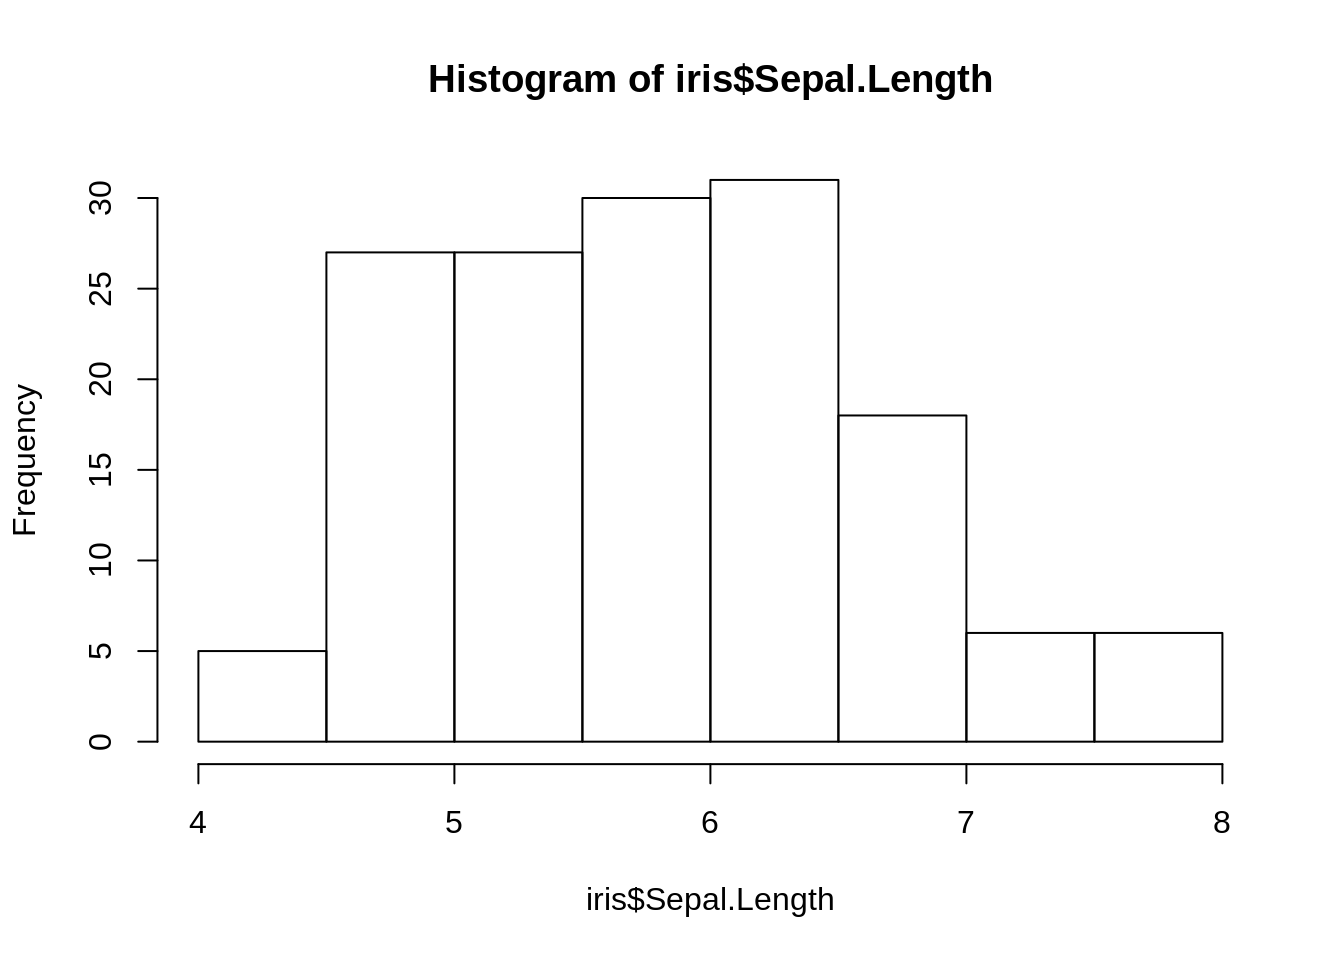
\includegraphics{BIOL416_Introduction_to_R_Notes_files/figure-latex/unnamed-chunk-29-1.pdf}

Easy, wasn't it? But it isn't very pretty - what could we change?

When we make modifications to our plot, we pass extra arguments. In the
original command, \texttt{hist(iris\$Sepal.Length)}, the only argument
we gave it was the data to plot.

Take a look at what other arguments are available with \texttt{?hist()}:

\begin{Shaded}
\begin{Highlighting}[]
\NormalTok{?}\KeywordTok{hist}\NormalTok{()}

\CommentTok{# Change the title, }\AlertTok{NOTICE}\CommentTok{ THAT WE USE COMMAS AND ARGUMENT NAMES!!!}
\KeywordTok{hist}\NormalTok{(}\DataTypeTok{x =}\NormalTok{ iris}\OperatorTok{$}\NormalTok{Sepal.Length, }\DataTypeTok{main =} \StringTok{"Observed frequency of sepal length"}\NormalTok{)}
\end{Highlighting}
\end{Shaded}

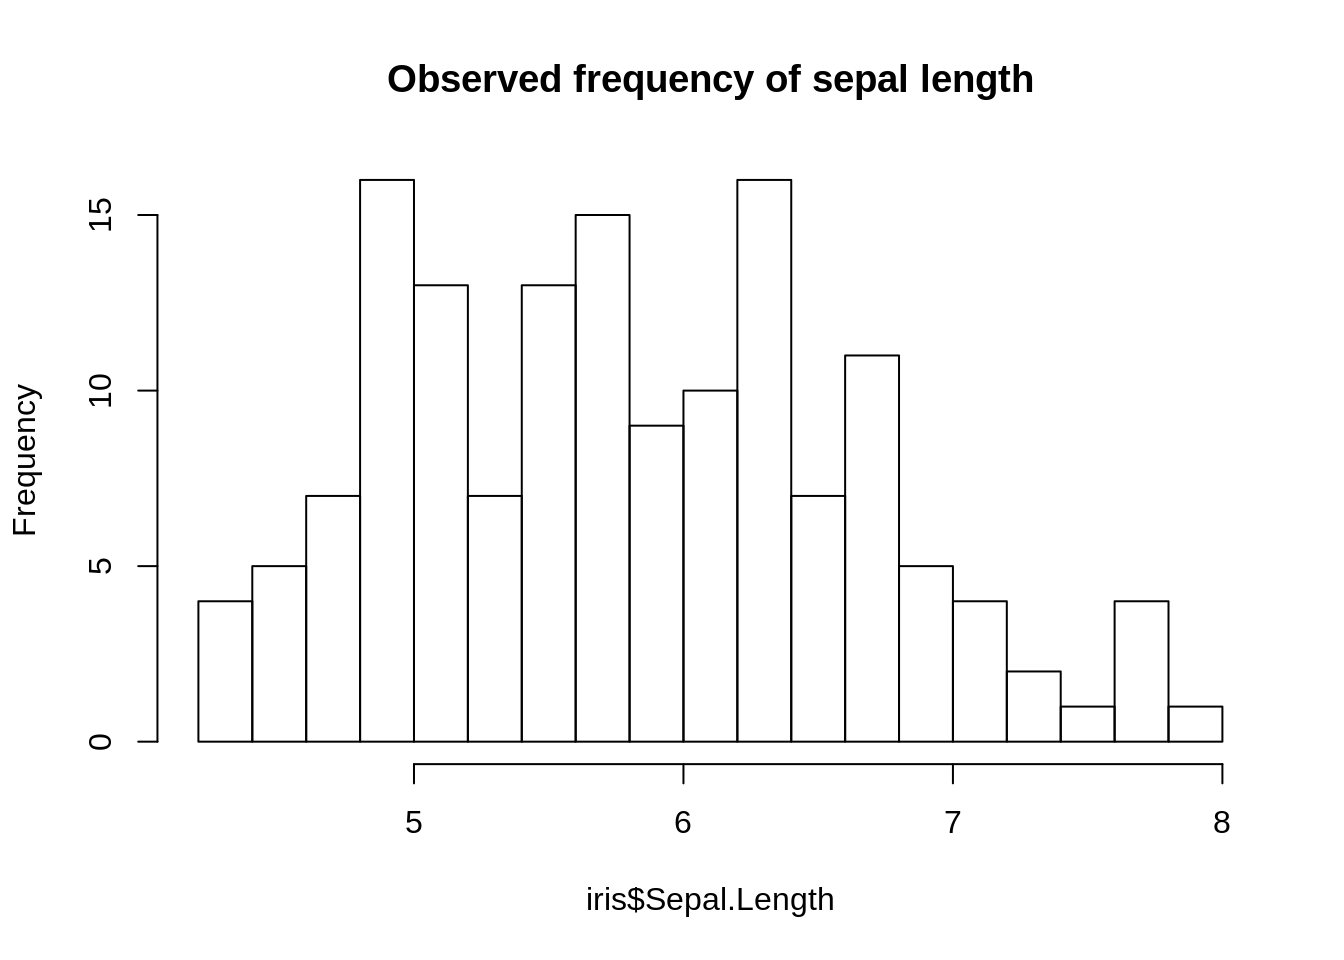
\includegraphics{BIOL416_Introduction_to_R_Notes_files/figure-latex/unnamed-chunk-30-1.pdf}

\begin{Shaded}
\begin{Highlighting}[]
\KeywordTok{hist}\NormalTok{(}\DataTypeTok{x =}\NormalTok{ iris}\OperatorTok{$}\NormalTok{Sepal.Length, }\DataTypeTok{main =} \StringTok{"Observed frequency of sepal length"}\NormalTok{, }\DataTypeTok{breaks =} \DecValTok{20}\NormalTok{)}
\end{Highlighting}
\end{Shaded}

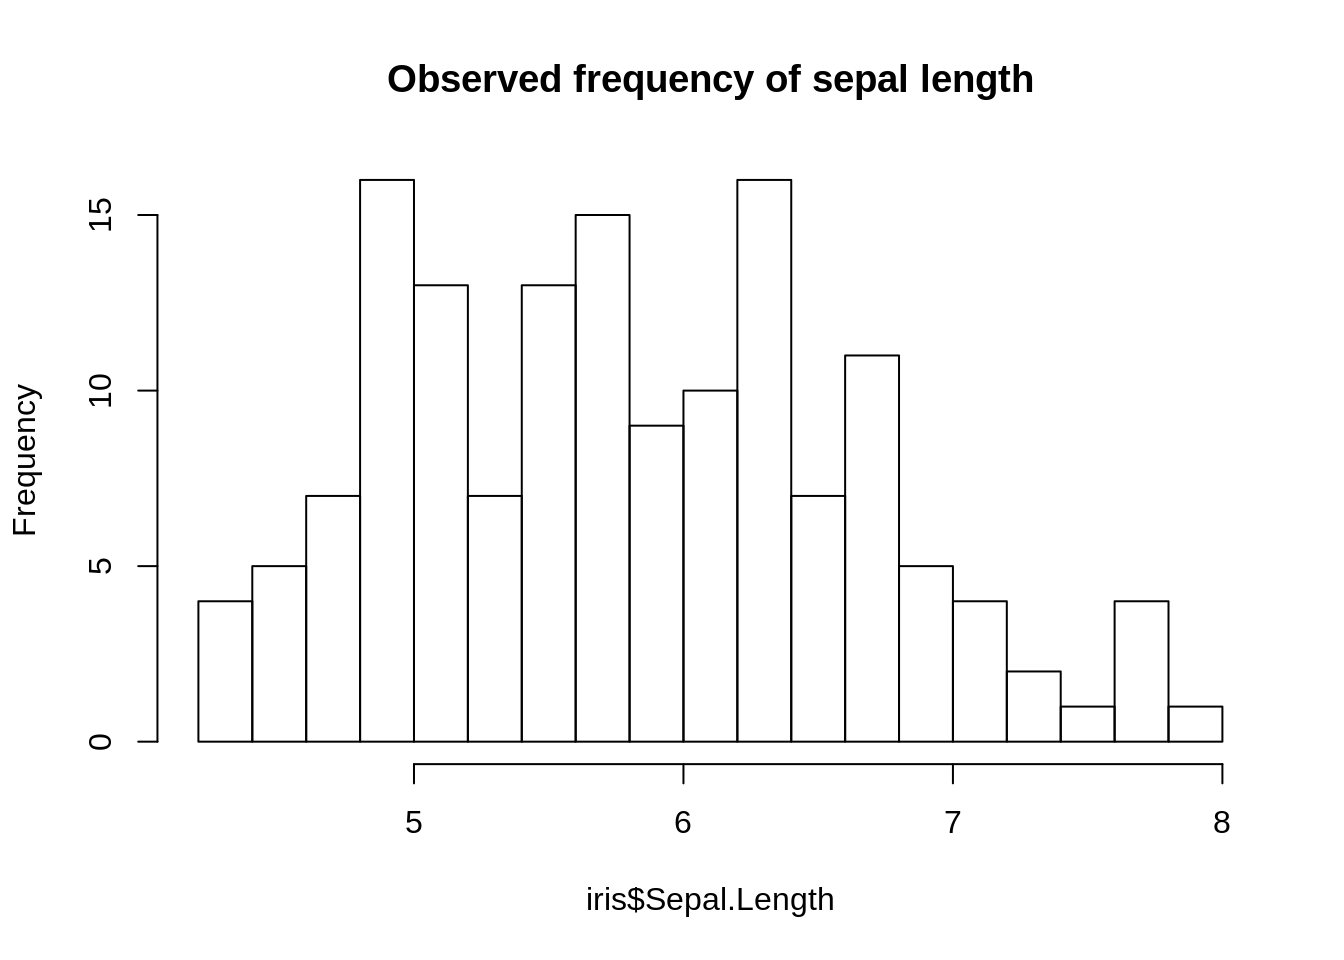
\includegraphics{BIOL416_Introduction_to_R_Notes_files/figure-latex/unnamed-chunk-31-1.pdf}

\begin{Shaded}
\begin{Highlighting}[]
\KeywordTok{hist}\NormalTok{(iris}\OperatorTok{$}\NormalTok{Sepal.Length, }
     \DataTypeTok{main =} \StringTok{"Observed frequency of sepal length"}\NormalTok{, }
     \DataTypeTok{breaks =} \DecValTok{20}\NormalTok{, }
     \DataTypeTok{xlab =} \StringTok{"Sepal Length (cm)"}\NormalTok{)}
\end{Highlighting}
\end{Shaded}

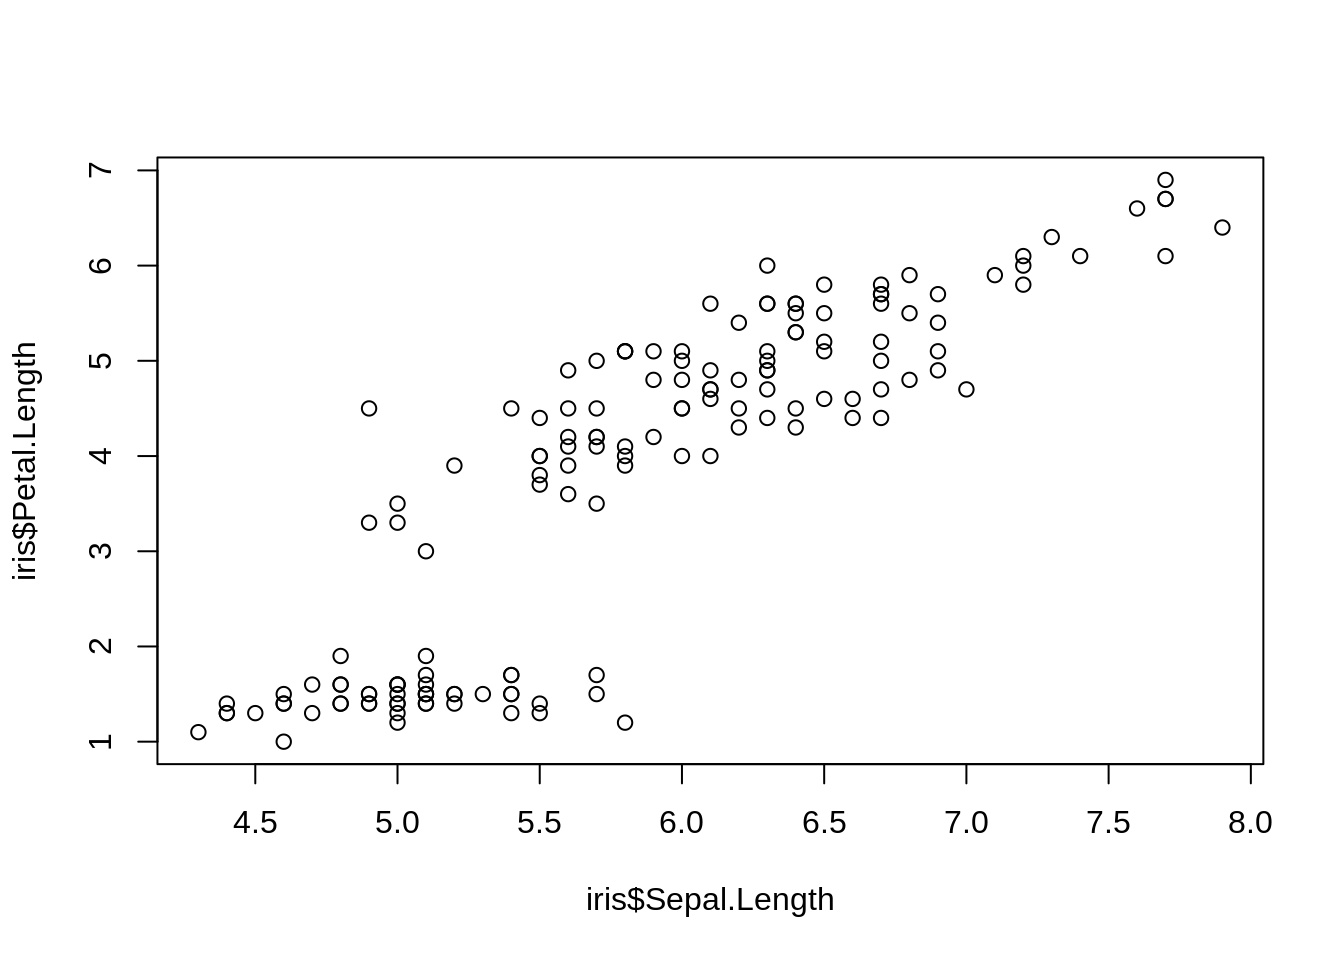
\includegraphics{BIOL416_Introduction_to_R_Notes_files/figure-latex/unnamed-chunk-32-1.pdf}

\subsubsection{Scatterplot}\label{scatterplot}

What about a more complicated type of plot next?

Let's try an x-y/scatter plot:

\begin{Shaded}
\begin{Highlighting}[]
\NormalTok{?}\KeywordTok{plot}\NormalTok{()}

\KeywordTok{plot}\NormalTok{(}\DataTypeTok{x =}\NormalTok{ iris}\OperatorTok{$}\NormalTok{Sepal.Length, }
     \DataTypeTok{y =}\NormalTok{ iris}\OperatorTok{$}\NormalTok{Petal.Length)}
\end{Highlighting}
\end{Shaded}

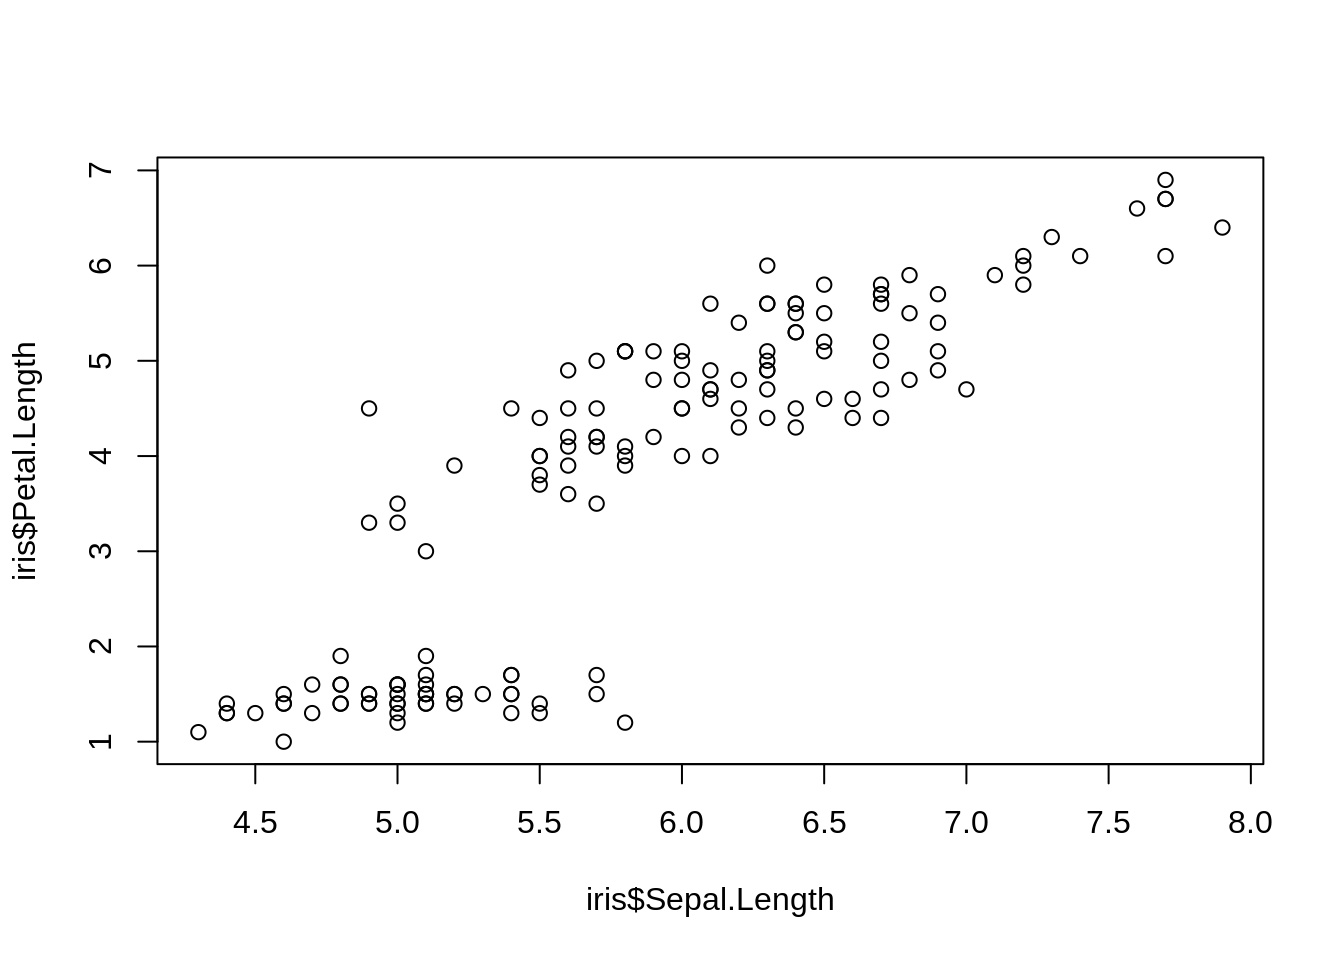
\includegraphics{BIOL416_Introduction_to_R_Notes_files/figure-latex/unnamed-chunk-33-1.pdf}

Take five minutes to change the main title and the X and Y axes' titles.

\begin{Shaded}
\begin{Highlighting}[]
\CommentTok{# Output should look something like this}
\KeywordTok{plot}\NormalTok{(}\DataTypeTok{x =}\NormalTok{ iris}\OperatorTok{$}\NormalTok{Sepal.Length, }
     \DataTypeTok{y =}\NormalTok{ iris}\OperatorTok{$}\NormalTok{Petal.Length,}
     \DataTypeTok{main =} \StringTok{"Iris sepal and petal dimensions"}\NormalTok{,}
     \DataTypeTok{ylab =} \StringTok{"Petal length (cm)"}\NormalTok{,}
     \DataTypeTok{xlab =} \StringTok{"Sepal length (cm)"}\NormalTok{)}
\end{Highlighting}
\end{Shaded}

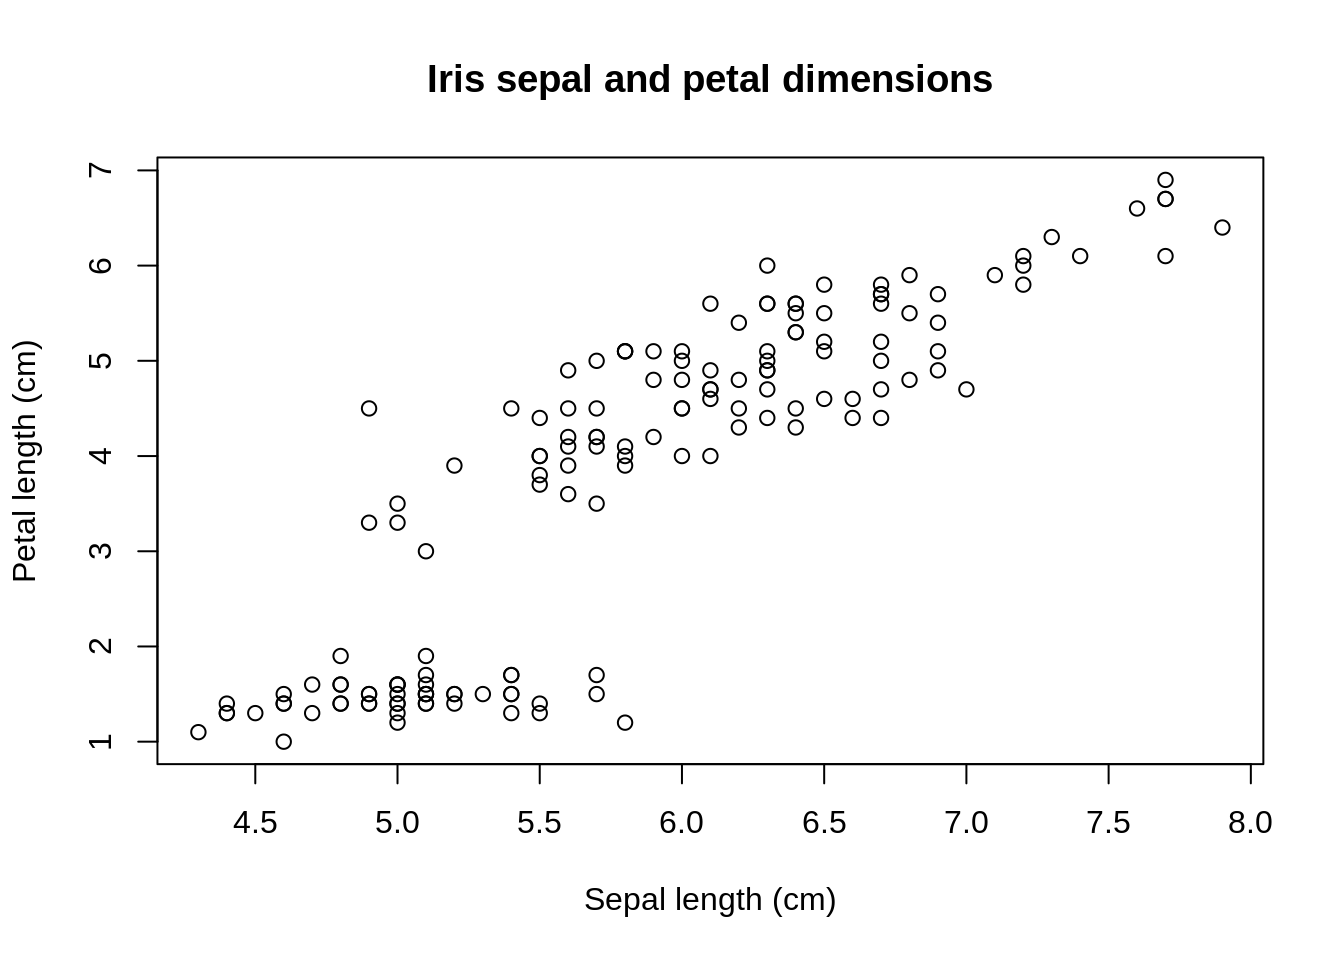
\includegraphics{BIOL416_Introduction_to_R_Notes_files/figure-latex/unnamed-chunk-34-1.pdf}

We can also goof around with colors and point types:

\begin{Shaded}
\begin{Highlighting}[]
\KeywordTok{plot}\NormalTok{(}\DataTypeTok{x =}\NormalTok{ iris}\OperatorTok{$}\NormalTok{Sepal.Length, }
     \DataTypeTok{y =}\NormalTok{ iris}\OperatorTok{$}\NormalTok{Petal.Length,}
     \DataTypeTok{main =} \StringTok{"Iris sepal and petal dimensions"}\NormalTok{,}
     \DataTypeTok{ylab =} \StringTok{"Petal length (cm)"}\NormalTok{,}
     \DataTypeTok{xlab =} \StringTok{"Sepal length (cm)"}\NormalTok{,}
     \DataTypeTok{col =}\NormalTok{ iris}\OperatorTok{$}\NormalTok{Species)}
\CommentTok{#     pch = 19)}

\CommentTok{# And we can add a legend:}
\KeywordTok{legend}\NormalTok{(}\DataTypeTok{x =} \FloatTok{4.2}\NormalTok{,}
       \DataTypeTok{y =} \DecValTok{7}\NormalTok{, }
       \DataTypeTok{legend =} \KeywordTok{unique}\NormalTok{(iris}\OperatorTok{$}\NormalTok{Species),}
       \DataTypeTok{fill =} \KeywordTok{c}\NormalTok{(}\StringTok{'black'}\NormalTok{,}\StringTok{'red'}\NormalTok{,}\StringTok{'green'}\NormalTok{))}
\end{Highlighting}
\end{Shaded}

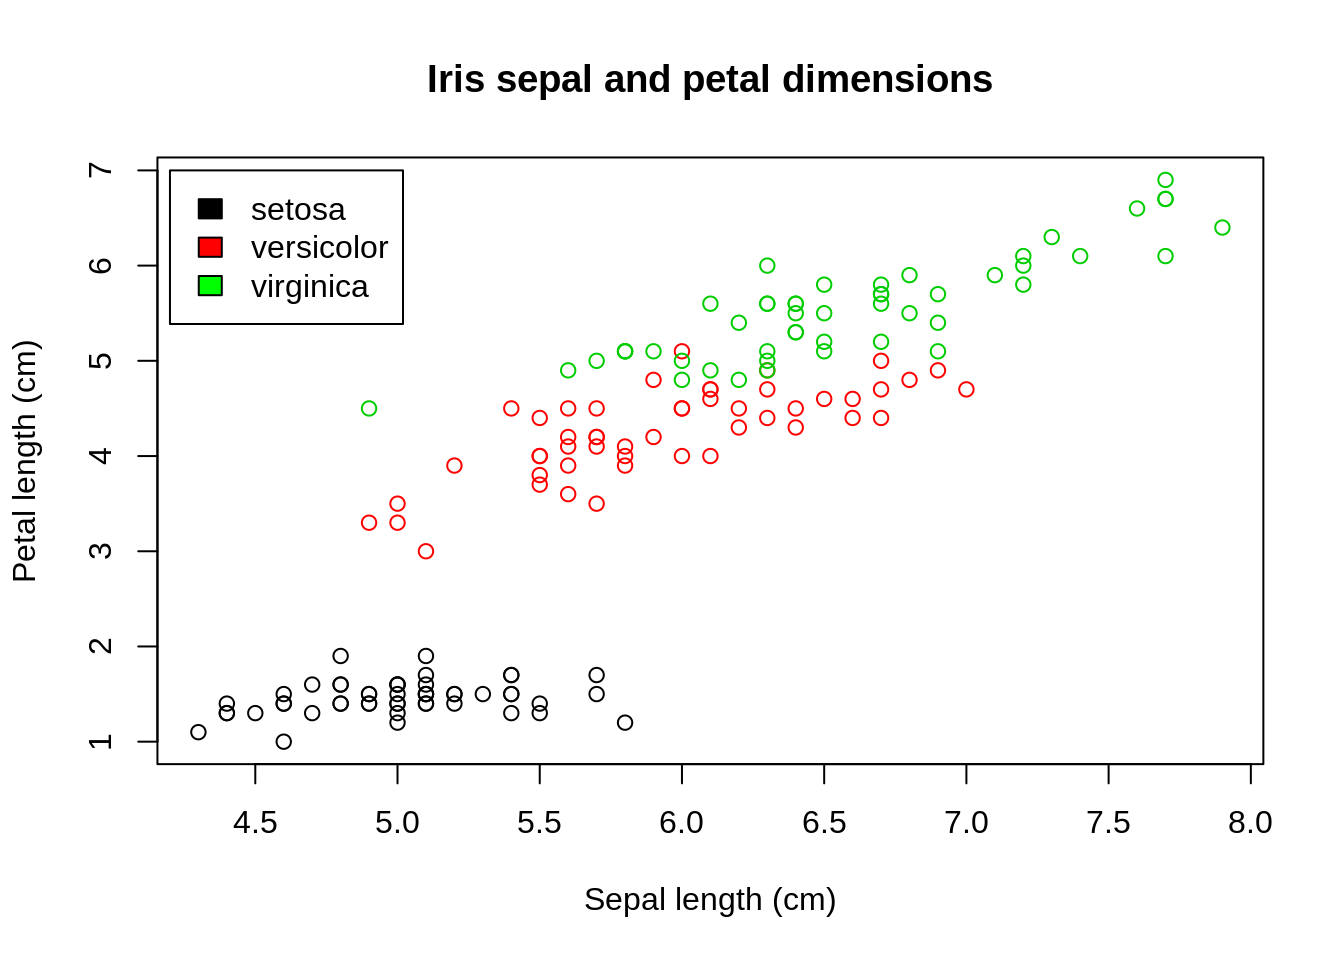
\includegraphics{BIOL416_Introduction_to_R_Notes_files/figure-latex/unnamed-chunk-35-1.pdf}

\subsubsection{Saving plots}\label{saving-plots}

Plots that you create in R can be saved in one of two ways:

\begin{enumerate}
\def\labelenumi{\arabic{enumi}.}
\tightlist
\item
  Saving in the \texttt{Plots} tab in the lower right panel
\item
  Saving directly in the code - most useful if you're going to be
  recreating the plots a bunch
\end{enumerate}

Here's how you save the image with code:

\begin{Shaded}
\begin{Highlighting}[]
\CommentTok{# Saving plots with code:}
\NormalTok{## For example, to save a .png:}
\KeywordTok{png}\NormalTok{(}\StringTok{"iris_scatterplot.png"}\NormalTok{)}
\KeywordTok{plot}\NormalTok{(}\DataTypeTok{x =}\NormalTok{ iris}\OperatorTok{$}\NormalTok{Sepal.Length, }
     \DataTypeTok{y =}\NormalTok{ iris}\OperatorTok{$}\NormalTok{Petal.Length,}
     \DataTypeTok{main =} \StringTok{"Iris sepal and petal dimensions"}\NormalTok{,}
     \DataTypeTok{ylab =} \StringTok{"Petal length (cm)"}\NormalTok{,}
     \DataTypeTok{xlab =} \StringTok{"Sepal length (cm)"}\NormalTok{,}
     \DataTypeTok{col =}\NormalTok{ iris}\OperatorTok{$}\NormalTok{Species,}
     \DataTypeTok{pch =} \DecValTok{19}\NormalTok{)}
\KeywordTok{dev.off}\NormalTok{()}
\end{Highlighting}
\end{Shaded}

\begin{verbatim}
## pdf 
##   2
\end{verbatim}

This uses two new functions:

\begin{itemize}
\tightlist
\item
  \texttt{png()} tells R to prepare a .png file with the name you
  provide
\item
  then, running \texttt{iris.scatterplot} prints out the plot within
  that file
\item
  finally, \texttt{dev.off()} closes the file and saves it
\end{itemize}

You can also save to other formats:

\begin{Shaded}
\begin{Highlighting}[]
\KeywordTok{pdf}\NormalTok{(}\StringTok{"iris_scatterplot.pdf"}\NormalTok{)}
\KeywordTok{plot}\NormalTok{(}\DataTypeTok{x =}\NormalTok{ iris}\OperatorTok{$}\NormalTok{Sepal.Length, }
     \DataTypeTok{y =}\NormalTok{ iris}\OperatorTok{$}\NormalTok{Petal.Length,}
     \DataTypeTok{main =} \StringTok{"Iris sepal and petal dimensions"}\NormalTok{,}
     \DataTypeTok{ylab =} \StringTok{"Petal length (cm)"}\NormalTok{,}
     \DataTypeTok{xlab =} \StringTok{"Sepal length (cm)"}\NormalTok{,}
     \DataTypeTok{col =}\NormalTok{ iris}\OperatorTok{$}\NormalTok{Species,}
     \DataTypeTok{pch =} \DecValTok{19}\NormalTok{)}
\KeywordTok{dev.off}\NormalTok{()}
\end{Highlighting}
\end{Shaded}

\begin{verbatim}
## pdf 
##   2
\end{verbatim}

\begin{Shaded}
\begin{Highlighting}[]
\CommentTok{# Or pass arguments about the plot itself, like the size, resolution, etc.}
\KeywordTok{png}\NormalTok{(}\StringTok{"iris_scatterplot_smaller.png"}\NormalTok{, }\DataTypeTok{width =} \DecValTok{200}\NormalTok{, }\DataTypeTok{height =} \DecValTok{200}\NormalTok{)}
\KeywordTok{plot}\NormalTok{(}\DataTypeTok{x =}\NormalTok{ iris}\OperatorTok{$}\NormalTok{Sepal.Length, }
     \DataTypeTok{y =}\NormalTok{ iris}\OperatorTok{$}\NormalTok{Petal.Length,}
     \DataTypeTok{main =} \StringTok{"Iris sepal and petal dimensions"}\NormalTok{,}
     \DataTypeTok{ylab =} \StringTok{"Petal length (cm)"}\NormalTok{,}
     \DataTypeTok{xlab =} \StringTok{"Sepal length (cm)"}\NormalTok{,}
     \DataTypeTok{col =}\NormalTok{ iris}\OperatorTok{$}\NormalTok{Species,}
     \DataTypeTok{pch =} \DecValTok{19}\NormalTok{)}
\KeywordTok{dev.off}\NormalTok{()}
\end{Highlighting}
\end{Shaded}

\begin{verbatim}
## pdf 
##   2
\end{verbatim}

Here's another type of plot - try to make this one on your own.

\begin{Shaded}
\begin{Highlighting}[]
\NormalTok{?}\KeywordTok{boxplot}\NormalTok{()}

\KeywordTok{boxplot}\NormalTok{(iris}\OperatorTok{$}\NormalTok{Sepal.Length}\OperatorTok{~}\NormalTok{iris}\OperatorTok{$}\NormalTok{Species, }\DataTypeTok{fill=}\NormalTok{iris}\OperatorTok{$}\NormalTok{Species,}
        \DataTypeTok{main =} \StringTok{"Boxplot of sepal length by species"}\NormalTok{,}
        \DataTypeTok{ylab =} \StringTok{"Sepal length (cm)"}\NormalTok{,}
        \DataTypeTok{xlab =} \StringTok{"Species"}
\NormalTok{)}
\end{Highlighting}
\end{Shaded}

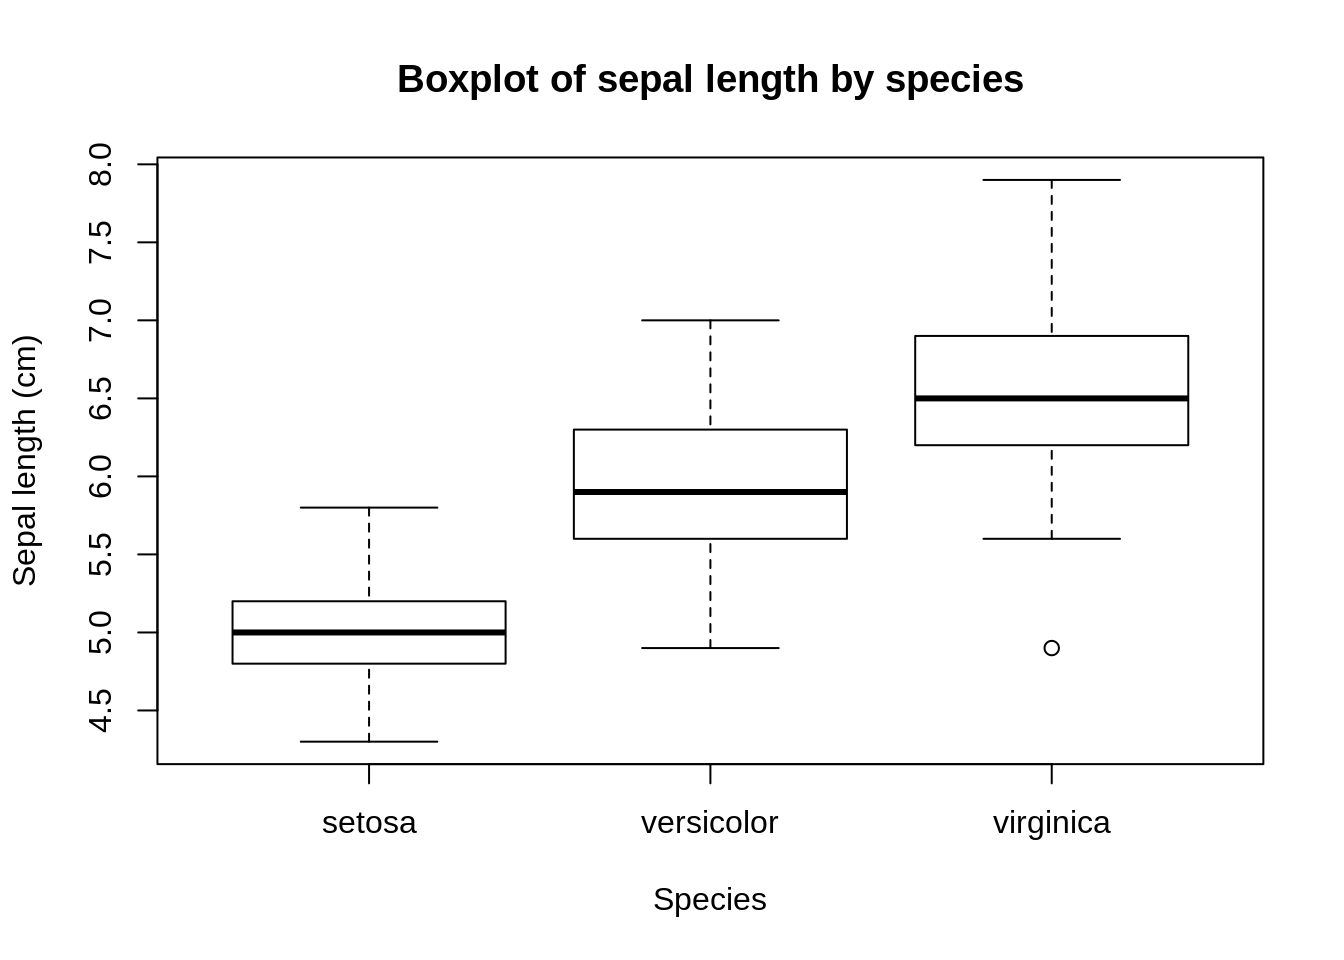
\includegraphics{BIOL416_Introduction_to_R_Notes_files/figure-latex/unnamed-chunk-38-1.pdf}

\subsubsection{Intro to statistics - linear
regression}\label{intro-to-statistics---linear-regression}

The final thing that R is particularly good at besides plotting data
performing statistics on those data.

Let's start with something really simple - what if we want to know how
correlated sepal length and petal length are in these three species of
iris? This is also useful for overlaying a line on top of our
scatterplot.

The tool that we want is called linear regression using a new function,
\texttt{lm()}.

\texttt{lm()} stands for linear model - this function fits a linear
regression between two variables. Essentially, linear regression is used
to calculate how closely correlated one variable is to another.

The linear part refers to the fact that we are calculating a
straight-line relationship between these two, just like in the classic
linear equation: \[ y = mx+b\]

If our \(x\) is sepal length and our \(y\) is petal length, we want to
create an equation that we can use to predict petal length based on some
observed sepal length.

In other words, we're asking ``when observed sepal length increases, how
much of an increase in petal length should we expect?'' We probably also
want to know if there is a statistically significant relationship
between the two, or if the trend we see in this plot could arise from
random noise in our data.

Linear regression finds the values for \(m\), the slope of the
relationship, and \(b\), the y-intercept of the line, that best predict
petal length from sepal length.

We're not going to go too much further into the statistical basis for
this, so let's just dive into the code.

\begin{Shaded}
\begin{Highlighting}[]
\CommentTok{# Regress petal length against sepal length}

\NormalTok{?}\KeywordTok{lm}\NormalTok{()}

\CommentTok{# lm() looks for a formula; in other words, we need to provide an equation for what variables we expect to be dependent on the other. }
\CommentTok{# In this case, let's assume that we are testing the petal length as a function of sepal length. }

\CommentTok{# }\AlertTok{NOTE}\CommentTok{: new argument, data =, allows us to use just the variable names directly}

\NormalTok{linear.model <-}\StringTok{ }\KeywordTok{lm}\NormalTok{(Petal.Length}\OperatorTok{~}\NormalTok{Sepal.Length,}
   \DataTypeTok{data =}\NormalTok{ iris)}

\KeywordTok{summary}\NormalTok{(linear.model)}
\end{Highlighting}
\end{Shaded}

\begin{verbatim}
## 
## Call:
## lm(formula = Petal.Length ~ Sepal.Length, data = iris)
## 
## Residuals:
##      Min       1Q   Median       3Q      Max 
## -2.47747 -0.59072 -0.00668  0.60484  2.49512 
## 
## Coefficients:
##              Estimate Std. Error t value Pr(>|t|)    
## (Intercept)  -7.10144    0.50666  -14.02   <2e-16 ***
## Sepal.Length  1.85843    0.08586   21.65   <2e-16 ***
## ---
## Signif. codes:  0 '***' 0.001 '**' 0.01 '*' 0.05 '.' 0.1 ' ' 1
## 
## Residual standard error: 0.8678 on 148 degrees of freedom
## Multiple R-squared:   0.76,  Adjusted R-squared:  0.7583 
## F-statistic: 468.6 on 1 and 148 DF,  p-value: < 2.2e-16
\end{verbatim}

Using the \texttt{summary()} command, R will spit out a bunch of
information about the results of our linear regression.

For example, the coefficient for \texttt{Sepal.Length} is 1.85843 - this
is the \(m\) value in our classical linear equation. Meanwhile, the
estimate for our y-intercept is -7.10144. Putting these into our
equation, we can say that the best linear equation to describe the
relationship between petal length and sepal length is:

\[
Petal.Length = 1.85843*Sepal.Length -7.10144
\] Now that we have this line, we can put it on top of our scatter plot!

\begin{Shaded}
\begin{Highlighting}[]
\CommentTok{# the abline() function can be used to directly put linear model objects onto a plot}
\KeywordTok{plot}\NormalTok{(}\DataTypeTok{x =}\NormalTok{ iris}\OperatorTok{$}\NormalTok{Sepal.Length, }
     \DataTypeTok{y =}\NormalTok{ iris}\OperatorTok{$}\NormalTok{Petal.Length,}
     \DataTypeTok{main =} \StringTok{"Iris sepal and petal dimensions"}\NormalTok{,}
     \DataTypeTok{ylab =} \StringTok{"Petal length (cm)"}\NormalTok{,}
     \DataTypeTok{xlab =} \StringTok{"Sepal length (cm)"}\NormalTok{,}
     \DataTypeTok{col =}\NormalTok{ iris}\OperatorTok{$}\NormalTok{Species)}\CommentTok{# ,}
     \CommentTok{#pch = 19)}
\KeywordTok{abline}\NormalTok{(linear.model)}
\KeywordTok{legend}\NormalTok{(}\DataTypeTok{x =} \FloatTok{4.2}\NormalTok{,}
       \DataTypeTok{y =} \DecValTok{7}\NormalTok{, }
       \DataTypeTok{legend =} \KeywordTok{unique}\NormalTok{(iris}\OperatorTok{$}\NormalTok{Species),}
       \DataTypeTok{fill =} \KeywordTok{c}\NormalTok{(}\StringTok{'black'}\NormalTok{,}\StringTok{'red'}\NormalTok{,}\StringTok{'green'}\NormalTok{))}
\end{Highlighting}
\end{Shaded}

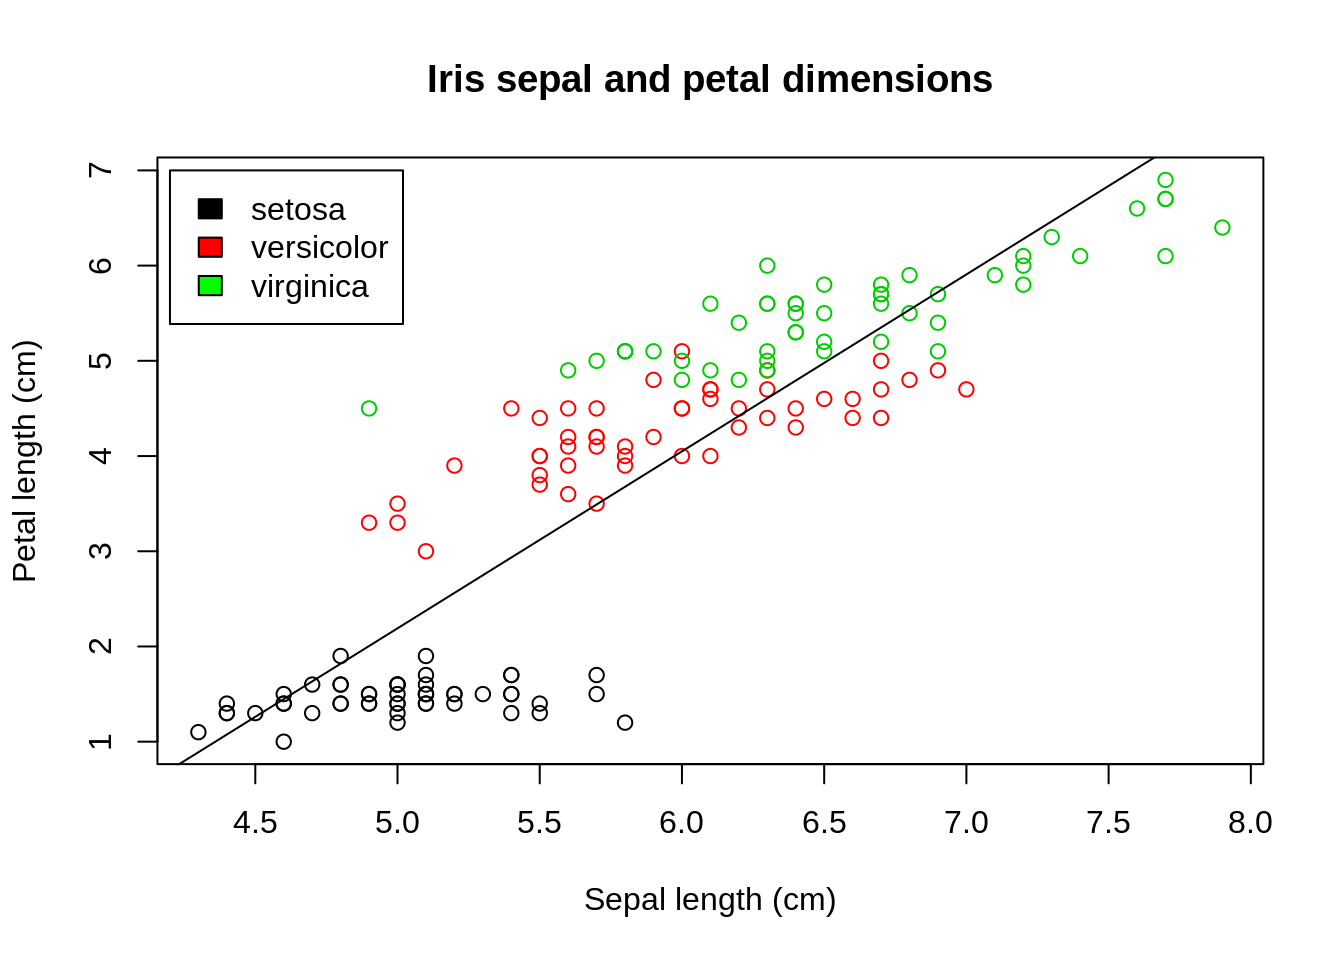
\includegraphics{BIOL416_Introduction_to_R_Notes_files/figure-latex/unnamed-chunk-40-1.pdf}


\end{document}
